% P17 — WORKING CHAPTER. Source-based reconstruction from frozen aggregates.
% Read report/README.md for provenance. NOT COMPILED / NOT FULL REPORT.
% Integrate with the institutional report template only after its original copy is preserved.
\chapter{Kết quả thực nghiệm và thảo luận}
\label{chap:ket-qua-thao-luan}

\section{Phạm vi đánh giá và cách đọc các chỉ số}
\label{sec:pham-vi-ket-qua}

Các kết quả trong chương này là các số liệu đã lưu của bài toán phát hiện xâm nhập nhị phân trên UNSW-NB15, với \textbf{Normal = 0} và \textbf{Attack = 1}. Tập huấn luyện chính thức có 175\,341 dòng và tập kiểm thử chính thức có 82\,332 dòng, gồm 37\,000 Normal và 45\,332 Attack. Ba pipeline được khóa trước đánh giá cuối là Random Forest 42 đặc trưng (RF-42), Stacking 42 đặc trưng (Stacking-42), và Random Forest 17 đặc trưng (RF-17). Tất cả sử dụng ngưỡng dự đoán nhị phân 0,5.

Các biến \texttt{id}, \texttt{label}, \texttt{attack\_cat} không được dùng làm biến dự đoán của bài toán nhị phân. \texttt{attack\_cat} chỉ được dùng để phân tích hậu nghiệm nhóm mẫu tấn công bị bỏ sót. Phần kết quả này \emph{không} chứng minh khả năng nhận diện đa lớp.

Với Attack là lớp dương, ta có:
\begin{equation}
  \mathrm{FPR}=\frac{\mathrm{FP}}{\mathrm{TN}+\mathrm{FP}},
  \qquad
  \mathrm{FNR}=\frac{\mathrm{FN}}{\mathrm{TP}+\mathrm{FN}},
  \qquad
  \mathrm{Detection\ Rate}=1-\mathrm{FNR}.
\end{equation}
Macro-F1 là trung bình F1 hai lớp với trọng số bằng nhau; MCC phản ánh tương quan giữa dự đoán và nhãn trong toàn bộ confusion matrix. Do có đánh đổi giữa báo động giả và bỏ sót, không nên dùng Accuracy riêng lẻ để kết luận mô hình tốt hơn.

\section{Kết quả trên official holdout}
\label{sec:ket-qua-official}

\begin{table}[htbp]
\centering
\small
\caption{Hiệu năng nhị phân của ba pipeline trên official TEST (82\,332 mẫu; threshold 0,5). FPR và FNR tính theo phần trăm.}
\label{tab:ket-qua-official}
\begin{tabular}{lrrrrrr}
\hline
Pipeline & Macro-F1 & MCC & FPR (\%) & FNR (\%) & FP & FN \\
\hline
RF-42       & 0.863343 & 0.750910 & 27.0351 & 1.6192 & 10003 & 734 \\
Stacking-42 & 0.863840 & 0.750497 & 26.6514 & 1.8795 & 9861 & 852 \\
RF-17       & 0.860673 & 0.746881 & 27.6324 & 1.5618 & 10224 & 708 \\
\hline
\end{tabular}
\end{table}

Stacking-42 có Macro-F1 nhỉnh hơn RF-42 về mặt số học, nhưng MCC thấp hơn rất nhẹ. Quan trọng hơn, Stacking-42 giảm \textbf{142 FP} (10\,003 xuống 9\,861) đồng thời tăng \textbf{118 FN} (734 lên 852). Đây là sự dịch chuyển đánh đổi giữa hai loại lỗi; chưa có ma trận chi phí tác nghiệp để quy đổi hai thay đổi này thành một lợi ích triển khai tổng thể.

RF-17 có Macro-F1 thấp hơn RF-42 khoảng 0,002670; đổi lại, thời gian và dung lượng mô hình lịch sử giảm đáng kể (Mục~\ref{sec:chi-phi}). RF-17 đồng thời sử dụng siêu tham số Random Forest khác RF-42, nên so sánh này là \emph{đánh đổi giữa hai pipeline}, không phải thí nghiệm chỉ thay duy nhất số đặc trưng.

\begin{figure}[htbp]
\centering
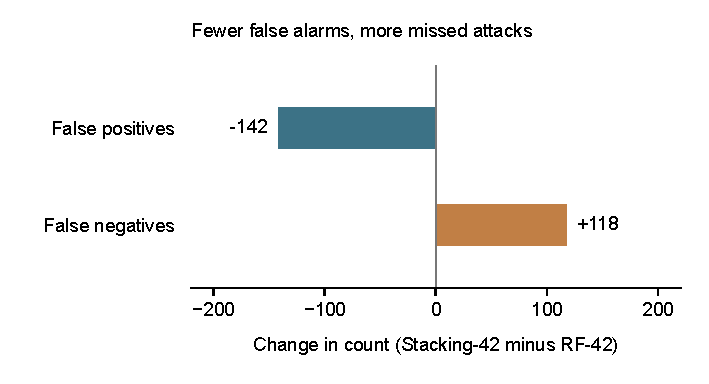
\includegraphics[width=0.82\textwidth]{../results/figures/p16_r05_error_tradeoff/error_tradeoff.pdf}
\caption{Chênh lệch số lượng lỗi Stacking-42 trừ RF-42 trên cùng official TEST: FP giảm 142 mẫu và FN tăng 118 mẫu. Số lượng quan sát trên benchmark cố định, không phải sai khác trung bình qua nhiều lần huấn luyện.}
\label{fig:delta-fp-fn}
\end{figure}

\section{Khoảng tin cậy và kiểm định cặp}
\label{sec:bat-dinh}

\begin{table}[htbp]
\centering
\small
\caption{Chênh lệch Stacking-42 trừ RF-42 và CI 95\% paired bootstrap đã lưu; 10\,000 lần lấy mẫu bootstrap từ các dòng benchmark. Đơn vị là độ chênh tuyệt đối trên thang 0--1.}
\label{tab:chenh-lech-ci}
\begin{tabular}{lrrr}
\hline
Chỉ số & $\Delta$ & CI dưới 95\% & CI trên 95\% \\
\hline
Macro-F1 & +0.000497 & -0.000312 & +0.001309 \\
MCC      & -0.000413 & -0.001938 & +0.001140 \\
FPR      & -0.003838 & -0.005243 & -0.002432 \\
FNR      & +0.002603 & +0.001853 & +0.003375 \\
\hline
\end{tabular}
\end{table}

Khoảng tin cậy của chênh lệch Macro-F1 và MCC chứa 0. Do đó, kết quả \emph{không cung cấp bằng chứng đủ mạnh cho ưu thế tổng thể} của Stacking-42 so với RF-42 trên hai thước đo này; điều này \emph{không} chứng minh hai mô hình tương đương thống kê. McNemar exact với hiệu chỉnh Holm trên \emph{đúng/sai tổng thể của các cặp dự đoán} cho $p_{\mathrm{Holm}}=0.468377$ trong cùng phép so sánh; McNemar không phải kiểm định trực tiếp chênh lệch Macro-F1.

CI của FPR nằm hoàn toàn phía âm và CI của FNR nằm hoàn toàn phía dương. Các khoảng tin cậy này phản ánh biến động do lấy mẫu lại \emph{các dòng benchmark đã lưu}, không phải độ ổn định qua các lần huấn luyện độc lập, session độc lập hay dữ liệu ngoài bộ UNSW-NB15. Hình forest plot và bảng số liệu nguồn được lưu trong \path{results/figures/p16_paired_effects_2026_10_16}.

\begin{figure}[htbp]
\centering
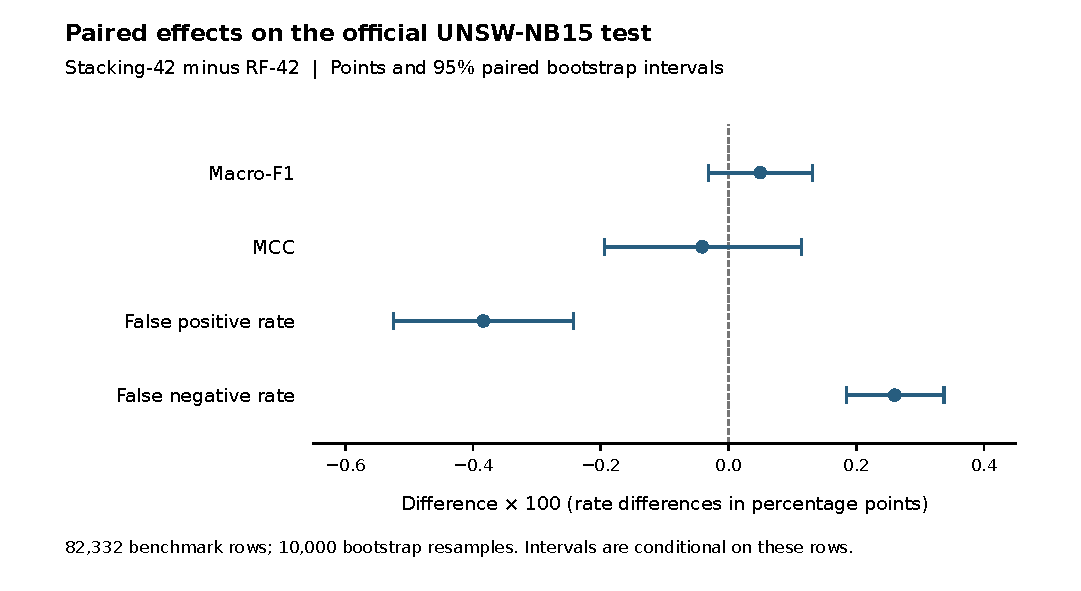
\includegraphics[width=0.95\textwidth]{../results/figures/p16_paired_effects_2026_10_16/paired_effects.pdf}
\caption{Bốn hiệu số Stacking-42 trừ RF-42 và CI 95\% paired bootstrap đã lưu. Giá trị trục ngang là hiệu số nhân 100 (không phải phần trăm thay đổi tương đối). CI của Macro-F1 và MCC chứa 0; FPR giảm, FNR tăng.}
\label{fig:paired-metrics}
\end{figure}

\section{Chi phí mô hình và số đặc trưng}
\label{sec:chi-phi}

\begin{table}[htbp]
\centering
\small
\caption{Chi phí được ghi nhận trong lần chạy lịch sử. Kích thước sử dụng đơn vị MiB (byte chia $1024^2$), không phải MB thập phân.}
\label{tab:chi-phi}
\begin{tabular}{lrrrr}
\hline
Pipeline & Số feature & Train (s) & Inference (ms/mẫu) & Size (MiB) \\
\hline
RF-42       & 42 & 371.244 & 0.008679 & 205.490 \\
Stacking-42 & 42 & 980.170 & 0.012445 & 206.216 \\
RF-17       & 17 & 57.255 & 0.003562 & 105.044 \\
\hline
\end{tabular}
\end{table}

Trong các số đo đã lưu, thời gian huấn luyện của RF-42 gấp khoảng 6,48 lần RF-17, và kích thước mô hình ước lượng của RF-17 thấp hơn khoảng 48,88\% so với RF-42. Các số liệu chỉ phản ánh \emph{chi phí quan sát của những cấu hình cụ thể trong lần chạy lịch sử}; chưa có phân bố thời gian qua nhiều lần huấn luyện và chưa có cơ sở dự báo thời gian trên thiết bị triển khai. Môi trường Python và thư viện tại thời điểm huấn luyện gốc chưa được xác định trực tiếp. Trường kích thước biểu diễn kết quả ước lượng serialize trong lần chạy, không chứng minh file mô hình cuối hiện tồn tại trên ổ đĩa.

\section{Phân tích lỗi theo họ tấn công}
\label{sec:attack-family-error}

\begin{table}[htbp]
\centering
\small
\caption{Số mẫu Attack thực bị dự đoán là Normal, phân nhóm theo \texttt{attack\_cat}; đây không phải đánh giá multiclass.}
\label{tab:attack-family}
\begin{tabular}{lrrrr}
\hline
Nhóm Attack & Số mẫu & FN RF-42 & FN Stack-42 & $\Delta$ FN \\
\hline
Fuzzers       & 6062  & 621 & 754 & +133 \\
Generic       & 18871 & 57  & 14  & -43 \\
Nhóm còn lại  & 20399 & 56  & 84  & +28 \\
\hline
Tổng Attack   & 45332 & 734 & 852 & +118 \\
\hline
\end{tabular}
\end{table}

Trên Fuzzers, Stacking-42 bỏ sót thêm 133 mẫu so với RF-42; trên Generic, Stacking-42 bỏ sót ít hơn 43 mẫu. Các đếm này mô tả tác động \emph{không đồng đều giữa các nhóm nhãn thật}, nhưng không chỉ ra cơ chế nhân quả của \texttt{sttl}, \texttt{proto} hay các feature khác. Những nhóm rất ít mẫu không cho phép khái quát chắc chắn về mọi tấn công ngoài benchmark. Tất cả phân tích lỗi được thực hiện hậu nghiệm trên prediction đã khóa, không được dùng để chỉnh ngưỡng dự đoán.

\section{Kiểm tra độ nhạy trên nhóm vector chưa trùng}
\label{sec:novel-vector}

\begin{table}[htbp]
\centering
\small
\caption{Macro-F1 trên official TEST và phần novel-vector của cùng official TEST. Novel-vector \emph{không} phải bộ dữ liệu kiểm thử độc lập.}
\label{tab:novel-vector}
\begin{tabular}{lrr}
\hline
Pipeline & Official TEST ($n=82332$) & Novel-vector ($n=73791$) \\
\hline
RF-42       & 0.863343 & 0.857473 \\
Stacking-42 & 0.863840 & 0.858125 \\
RF-17       & 0.860673 & 0.855723 \\
\hline
\end{tabular}
\end{table}

Cả ba pipeline có Macro-F1 thấp hơn trên nhóm novel-vector. Tập con này được xác định bằng cách loại những dòng TEST có vector 42 đặc trưng trùng với ít nhất một vector TRAIN; 8\,541 dòng TEST thuộc nhóm overlap theo cách định nghĩa này. Đây là một \emph{sensitivity analysis} trong cùng benchmark, không thay cho đánh giá external, temporal, day hoặc session split. Vì vậy, câu hỏi RQ4 về độ nhạy với \emph{split protocol} chưa được trả lời đầy đủ.

\section{Tổng hợp theo câu hỏi nghiên cứu và các giới hạn}
\label{sec:rq-limitations}

\textbf{RQ1 --- Hiệu quả ensemble:} chưa chứng minh cải thiện tổng thể hoặc ổn định qua nhiều lần huấn luyện của Stacking-42 so với RF-42. Kết quả cặp cho thấy dịch chuyển FP/FN rõ ràng trên holdout đã lưu.

\textbf{RQ2 --- Feature selection:} bảng so sánh RF-17 và RF-42 hỗ trợ mô tả đánh đổi hiệu năng--chi phí của \emph{cả pipeline}; không có đối chứng tách biệt tác động nhân quả của chỉ số feature vì cấu hình mô hình cũng khác nhau.

\textbf{RQ3 --- Complementarity:} các bảng OOF diversity và ensemble ở development hỗ trợ phân tích \emph{liên hệ mô tả} giữa sai số của base learners và kết quả kết hợp. Complementary errors không bảo đảm Stacking vượt mô hình đơn; các kết quả voting kém hơn vẫn phải được báo cáo.

\textbf{RQ4 --- Robustness:} novel-vector cho thấy một hướng kiểm tra độ nhạy nhưng không phải temporal/group/external validation. RQ4 mới được trả lời một phần.

\textbf{RQ5 phụ --- Class imbalance:} chưa có thí nghiệm controlled resampling so sánh matched, do đó không thể khẳng định SMOTE hay kỹ thuật sampling tương đương hiệu quả hoặc không hiệu quả trong nghiên cứu này.

\textbf{Giới hạn phương pháp:} (i) lựa chọn stable features trên toàn official TRAIN trước development CV có thể làm điểm CV lạc quan; (ii) lựa chọn/tuning meta-model chưa fully nested; (iii) có vector trùng giữa official TRAIN và TEST và các dòng network-flow không được chứng minh độc lập ở cấp session; (iv) paired bootstrap là trên dòng benchmark chứ không phải repeated-training stability; (v) môi trường training lịch sử chưa xác minh trực tiếp và chưa có final serialized model hợp lệ; (vi) không có kiểm tra external deployment/multiclass. Các giới hạn này không được xóa hoặc sửa kết quả official TEST sau khi đã quan sát.

\section{Kết luận chương}
Trong giới hạn official UNSW-NB15 holdout đã khóa, Stacking-42 làm giảm báo động giả nhưng đồng thời tăng số tấn công bị bỏ sót so với RF-42. Bằng chứng thống kê hiện có chưa xác nhận một cải thiện tổng thể về Macro-F1/MCC. RF-17 thể hiện khả năng giảm chi phí của một cấu hình pipeline khác với mức giảm nhỏ của Macro-F1. Giá trị khoa học hiện có nằm ở đối chiếu có truy vết, phân tích sai số, độ bất định và công bố giới hạn, thay vì tuyên bố một thuật toán ensemble mới hoặc khả năng triển khai ngoài benchmark đã được xác minh.
